% =====================================================================
%  ME 697 -- Class Project: 1-D Lagrangian Hydrocode      Equation sheet v4
%  v4 (Oct 19): Instructor's Note at the top (what bitwhiz is, the two
%  methods, AI assistance); text shared word for word with the RS sheet.
%  v3 notes follow.
%  Method AV (artificial viscosity).  rev-1 draft, Oct 19, 2026 (with Claude)
%
%  What v3 adds to v2 (= the published rev-0), for DK to accept or reject:
%    [5] Boxes titled "bitwhiz: ..." go BEYOND the project rules: they say
%        what the class reference code, bitwhiz, does.  The plain boxes are
%        still the project rules.  New bitwhiz boxes: Tension and Cell
%        Breaking (spall_strength, damage), Expansion Branch (the cubic),
%        and Where This Lives in bitwhiz (steps -> routines, symbols ->
%        database slots).  With spall_strength = 0 the pressure rule is the
%        project's P >= 0 rule.
%    [6] EOS box: P = rho0*Gamma0*e + Pi(V), the form bitwhiz evaluates;
%        P_H written as rho0*eta*U_S^2 (no 0/0 at V0); eta = (rho-rho0)/rho.
%        Pi is a new symbol (U3 already uses phi for transported quantities).
%    [7] Sound speed in the general form c^2 = V^2[rho0*Gamma0*P - dPi/dV],
%        evaluated at the pressure KEPT by the spall rule.
%    [8] Time step: CFL from the deck (default 0.6); the first and last
%        steps; a void cell's step.  One Cycle: the spall rule in step d.
%    [9] Boundary box: the end face's stress in the energy update is not
%        exactly zero while the end cell is being compressed (q_k/2): this
%        is what the formulas (and bitwhiz) give.  DK to decide.
%  Checked against bitwhiz 311bf6d: av_mod (face_step, cell_step,
%  cell_state, cell_dt), eos_mod (mg_ref), maincode sections 5-7.
%
%  ---- v1/v2 notes (Oct 7-8), kept for the record ----
%  ME 697 -- Class Project: 1-D Lagrangian Hydrocode      Equation sheet v1
%  Fall 2026, D. Kittell                                   drafted Oct 7
%
%  Source of record: Lecture 19 + its addendum (ME697_Lec19_2026-10-07_
%  Addendum.pdf, reposted Oct 8) and the project document v6.  Equations
%  only -- no derivations.  Notation follows the addendum (M_k, c_k,
%  half-integer faces) and Equation_Sheets/README.md.
%
%  Deliberate departures from the addendum, for DK to accept or reject:
%    [1] Units: x in mm, not cm.  With mm, us, g/cm^3, GPa, km/s, MJ/kg
%        every update below needs no conversion factor (cm needs 10x).
%    [2] CFL uses x^{n+1} and u^{n+1/2}; the addendum's x^{n+1/2} is never
%        computed by the scheme.
%    [3] Step 2 is the p. 3 boxed total-energy update (verified).  The
%        pp. 8-9 end line is NOT used -- it double counts the pressure work.
%    [4] Added: a note on variable time steps (Step 1), the de_H/dV identity
%        (sound speed), a momentum-weighted starting velocity on an impact
%        face, and a conservation check (One Cycle box).
%  Verified Oct 7 (python): sound speed vs brute-force isentrope for Al and
%  Material X (agree to 1e-9; c -> c0 at V0, e=0); Al/Al symmetric impact at
%  1 km/s, 35 zones/mm, B_L=0.1, B_Q=2, CFL 0.6: plateau P = 8.288 GPa vs
%  8.298 analytic (-0.12%), u = 0.500 km/s.
% =====================================================================

\documentclass[11pt,addpoints]{exam}
\usepackage{amsfonts,amssymb,amsmath, amsthm}
\usepackage{graphicx}
\usepackage{enumitem}
\usepackage{systeme}
\usepackage{pgf,tikz,pgfplots}
\pgfplotsset{compat=1.15}
\usepgfplotslibrary{fillbetween}
\usepackage{mathrsfs}
\usepackage{multicol}
\usepackage{booktabs}
\usepackage[many]{tcolorbox}
\usepackage{bm}
\usepackage{cancel}
\allowdisplaybreaks

% Good Volume Symbol
\newcommand{\volume}{{\ooalign{$V$\cr\hfil\raisebox{0.35em}{\rule{2.1mm}{0.1ex}}\hfil\cr}}}

%%% Strike-out font
\usepackage{ulem}
\normalem
\pagestyle{headandfoot}

% ---- Warm theme to match the figures (U5 onward) ----
\definecolor{slate}{HTML}{2C3E50}
\definecolor{oiblue}{HTML}{0072B2}
\tcbset{colback=oiblue!4!white, colframe=slate, boxrule=0.5pt, arc=1.5mm}

\firstpageheader{ME 697 Equations}{Class Project: Hydrocode, Method AV}{Fall 2026 -- D. Kittell}
\runningheader{ME 697 Equations}{Class Project: Hydrocode, Method AV}{Fall 2026 -- D. Kittell}
\runningheadrule
\firstpagefooter{}{}{}
\runningfooter{}{}{}

\makeatletter
\renewcommand*\env@matrix[1][*\c@MaxMatrixCols c]{%
  \hskip -\arraycolsep
  \let\@ifnextchar\new@ifnextchar
  \array{#1}}
\makeatother

\begin{document}

\noindent
\bf{Instructor's Note:}\normalfont\\

\noindent
\it{\texttt{bitwhiz} is the reference hydrocode for ME 697, Intermediate Shock and Detonation Theory (Purdue, Fall 2026): a one-dimensional, planar, Lagrangian code for plate impact, with shock and release waves crossing layers of solids and liquids, and spall where release waves meet in tension. Two solution methods share one code: this sheet is Method AV (artificial viscosity), and the companion sheet is Method RS (a Riemann solver). It was written by D.~Kittell with the assistance of Claude Opus 5.5 (Anthropic), an AI model; the instructor directed, reviewed, and tested every part of it and is responsible for its content.}\normalfont\vspace{1.5em}

\textbf{These equations build upon U3. Continuum Mechanics {\&} Balance Laws and the Lecture 19 Addendum (artificial viscosity method)}\vspace{1em}


\begin{tcolorbox}[breakable]
\textbf{Notation \& Scope:}\vspace{.5em}
\begin{itemize}
\item One-dimensional hydrocode, planar, Lagrangian, and purely hydrodynamic, such that \hspace{3mm} \bm{$\displaystyle \sigma_{xx}\;=\;-\left(P\;+\;q\right)$} \hspace{5mm} with \bm{$Y=0$} and artificial viscosity, \bm{$q$}\vspace{.5em}
\item Grid discretization has integers, \bm{$k$}, at cell \emph{centers}, and \bm{$k\pm\frac{1}{2}$} at \emph{faces}; \hspace{2mm} time step index is \bm{$n$}: whole and half steps considered, \bm{$\Delta t^n$} spans \bm{$n\rightarrow n+1$}\vspace{.5em}
\item Staggered Grid, \hspace{3mm} \bm{$u$}, \bm{$x$} \hspace{2mm} face-centered; \hspace{3mm} \bm{$\rho$}, \bm{$\text{V}=1/\rho$}, \bm{$e$}, \bm{$P$}, \bm{$q$}, \bm{$c$} \hspace{2mm} cell-centered\vspace{.5em}
\item Cell Mass, \hspace{3mm} \bm{$M_k$} \hspace{5mm} is mass per unit area of cell \bm{$k$}, fixed for all time \hspace{3mm} (note: the areal mass coordinate \bm{$h$} of U7 advances by \bm{$M_k$} per cell)\vspace{.5em}
\item Sound Speed, \hspace{3mm} \bm{$c_k$} \hspace{3mm} is the isentropic sound speed of cell \bm{$k$} (subscript \bm{$s$} dropped); \hspace{2mm} initial state is \bm{$\left(\;\;\right)_0$}, Hugoniot state is \bm{$\left(\;\;\right)_H$}\vspace{.5em}
\item Boxes titled \textbf{bitwhiz:} go beyond the \textbf{\emph{project rules}}, to what the reference code \texttt{bitwhiz} does
\end{itemize}
\end{tcolorbox}


\begin{tcolorbox}[breakable]
\textbf{A Consistent Set of Units (no conversion factors anywhere below):}\vspace{.5em}
\begin{itemize}
\item \bm{$x$} [mm], \hspace{2mm} \bm{$t$} [\bm{$\mu$}s], \hspace{2mm} \bm{$\rho$} [g/cm\bm{$^3$}], \hspace{2mm} \bm{$u,\;c$} [km/s] \bm{$=$} [mm/\bm{$\mu$}s], \hspace{2mm} \bm{$P,\;q$} [GPa], \hspace{2mm} \bm{$e$} [MJ/kg] \bm{$=$} [km\bm{$^2$}/s\bm{$^2$}]\vspace{.5em}
\item Cell Mass, \hspace{3mm} \bm{$M_k$} [g/cm\bm{$^3\cdot$}mm] \hspace{5mm} e.g., \bm{$\displaystyle \frac{\Delta t\,\Delta P}{M}\;\rightarrow\;\frac{[\mu\text{s}][\text{GPa}]}{[\text{g/cm}^3][\text{mm}]}\;=\;[\text{km/s}]$}\vspace{.5em}
\item If you stick to using these units, there won't be any conversion factors inside your code. If you change units, e.g., \bm{$x$} in [cm] instead, then there will be conversion factors.
\end{itemize}
\end{tcolorbox}

\clearpage

\begin{tcolorbox}[breakable]
\textbf{Step 0. Mesh and Initial Conditions:}\vspace{.5em}
\begin{itemize}
\item Faces, \hspace{3mm} \bm{$x^0_{k+\frac{1}{2}}$} \hspace{5mm} uniform within each material; adjust zones per material so that \textbf{\emph{every material interface lands on a cell face}}\vspace{.5em}
\item Cell Mass, \hspace{3mm} \bm{$\displaystyle M_k\;=\;\rho_{0,k}\left(x^0_{k+\frac{1}{2}}\;-\;x^0_{k-\frac{1}{2}}\right)$} \hspace{7mm} computed once, constant over time\vspace{.5em}
\item Cell State, \hspace{3mm} \bm{$\rho^0_k=\rho_{0,k}$}, \hspace{2mm} \bm{$e^0_k=0$}, \hspace{2mm} \bm{$P^0_k=0$}, \hspace{2mm} \bm{$q^0_k=0$}, \hspace{2mm} \bm{$c^0_k=c_{0,k}$}\vspace{.5em}
\item Face Velocity, \hspace{3mm} \bm{$u^{-\frac{1}{2}}_{k+\frac{1}{2}}$} \hspace{2mm} the initial velocity of the material on both sides; on an impact face you may use the momentum-weighted value \bm{$\displaystyle \frac{M_k u_{0,k}+M_{k+1}u_{0,k+1}}{M_k+M_{k+1}}$}
\end{itemize}
\end{tcolorbox}

\begin{figure}[h!]
  \centering
  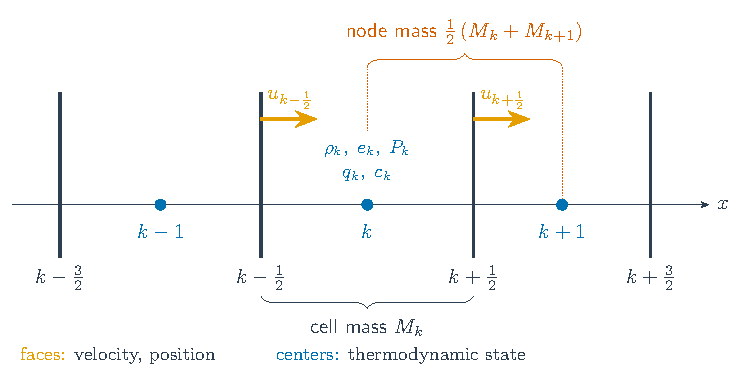
\includegraphics[width=0.66\textwidth]{hc_grid_v1.pdf}
  \caption{Staggered grid (cartoon). Velocity and position live on the faces; the thermodynamic state lives at the centers. The momentum update divides by the node mass, the cell-to-cell average shown in red.\label{fig:grid}}
\end{figure}

\clearpage


\begin{tcolorbox}[breakable]
\textbf{Step 1. Velocity, Position, and Density:}\vspace{.5em}
\begin{itemize}
\item Momentum, \hspace{3mm} for every face between cells \bm{$k$} and \bm{$k+1$}\vspace{.5em}\\
.~~~~~~~~~~\bm{$\displaystyle u^{n+\frac{1}{2}}_{k+\frac{1}{2}}\;=\;u^{n-\frac{1}{2}}_{k+\frac{1}{2}}\;+\;\frac{2\,\Delta t^n}{M_k+M_{k+1}}\left[\left(P^n_k-P^n_{k+1}\right)\;+\;\left(q^n_k-q^n_{k+1}\right)\right]$}\vspace{1em}
\item Cell Kinematics, \hspace{3mm} \bm{$\displaystyle x^{n+1}_{k+\frac{1}{2}}\;=\;x^{n}_{k+\frac{1}{2}}\;+\;u^{n+\frac{1}{2}}_{k+\frac{1}{2}}\,\Delta t^n$} \hspace{7mm} the mesh moves with mass\vspace{.5em}
\item Cell Density, \hspace{3mm} \bm{$\displaystyle \rho^{n+1}_k\;=\;\frac{M_k}{x^{n+1}_{k+\frac{1}{2}}\;-\;x^{n+1}_{k-\frac{1}{2}}}$} \hspace{7mm} and, if needed, \bm{$\text{V}^{n+1}_k=1/\rho^{n+1}_k$}\vspace{.5em}
\item Note: the velocity step spans \bm{$n-\frac{1}{2}\rightarrow n+\frac{1}{2}$}. With a fixed \bm{$\Delta t$} this is exactly \bm{$\Delta t^n$}; when \bm{$\Delta t$} changes every cycle, \bm{$\frac{1}{2}\left(\Delta t^{n-1}+\Delta t^n\right)$} is the time-centered choice (see Fig.~\ref{fig:leap})
\end{itemize}
\end{tcolorbox}

\begin{figure}[!ht]
  \centering
  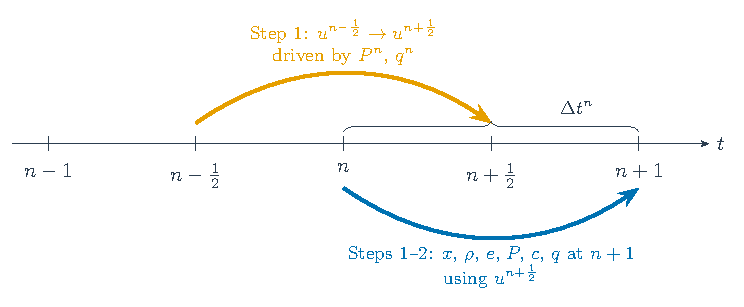
\includegraphics[width=0.58\textwidth]{hc_leapfrog_v1.pdf}
  \caption{Leapfrog time integration (cartoon). Velocity is advanced on half steps by the state at the whole step between them; everything else is advanced on whole steps by the new velocity.\label{fig:leap}}
\end{figure}

\clearpage


\begin{tcolorbox}[breakable]
\textbf{Step 2. Energy and Pressure:}\vspace{.5em}
\begin{itemize}
\item Total Energy (cell \bm{$k$}), \hspace{3mm} face stresses are mass-weighted, face viscosities averaged\vspace{.5em}\\
.~~~~\bm{$\displaystyle e^{n+1}_k\;=\;e^n_k\;+\;\frac{\Delta t^n}{M_k}\left[\frac{M_kP^n_{k-1}+M_{k-1}P^n_k}{M_k+M_{k-1}}\;+\;\frac{q^n_k+q^n_{k-1}}{2}\right]u^{n+\frac{1}{2}}_{k-\frac{1}{2}}$}\vspace{1em}\\
.~~~~~~~~~~~~~~~~\bm{$\displaystyle -\;\frac{\Delta t^n}{M_k}\left[\frac{M_{k+1}P^n_k+M_kP^n_{k+1}}{M_k+M_{k+1}}\;+\;\frac{q^n_k+q^n_{k+1}}{2}\right]u^{n+\frac{1}{2}}_{k+\frac{1}{2}}$}\vspace{1em}\\
.~~~~~~~~~~~~~~~~\bm{$\displaystyle +\;\frac{1}{8}\left[\left(u^{n-\frac{1}{2}}_{k+\frac{1}{2}}+u^{n-\frac{1}{2}}_{k-\frac{1}{2}}\right)^2\;-\;\left(u^{n+\frac{1}{2}}_{k+\frac{1}{2}}+u^{n+\frac{1}{2}}_{k-\frac{1}{2}}\right)^2\right]$}\vspace{1em}
\item Reading the terms: work done by the face stresses, minus the change in the cell's kinetic energy \bm{$\frac{1}{2}\bar{u}^2$}, with \bm{$\bar{u}=\frac{1}{2}\left(u_{k-\frac{1}{2}}+u_{k+\frac{1}{2}}\right)$} \hspace{2mm} \textbf{\emph{easiest place for mistakes}}\vspace{.5em}
\item Pressure, \hspace{3mm} \bm{$\displaystyle P^{n+1}_k\;=\;P\left(\rho^{n+1}_k,\;e^{n+1}_k\right)$} \hspace{7mm} from the equation of state of cell \bm{$k$}\vspace{.5em}
\item Pressure Bounds, \hspace{3mm} \bm{$P\;\ge\;0$} \hspace{5mm} flag the first cell that goes tensile and the time it happens, then set it to zero and continue (project Sec.~3; \texttt{bitwhiz}: see Tension and Cell Breaking)
\end{itemize}
\end{tcolorbox}

\clearpage


\begin{tcolorbox}[breakable]
\textbf{bitwhiz: Tension and Cell Breaking (Spall):}\vspace{.5em}
\begin{itemize}
\item Spall Strength, \hspace{3mm} \bm{$P_{sp}>0$} \hspace{2mm} per material (deck: \texttt{spall\_strength}, default 0.01 GPa); \hspace{3mm} Damage, \hspace{2mm} \bm{$\mathcal{D}_k=0$} intact, \bm{$\mathcal{D}_k=1$} broken; every cell starts intact\vspace{.5em}
\item Intact, \hspace{3mm} keep the EOS pressure while \hspace{2mm} \bm{$P^{n+1}_k\;\ge\;-P_{sp}$} \hspace{7mm} an intact cell \textbf{\emph{holds tension}}\vspace{.5em}
\item Breaking, \hspace{3mm} if intact and \hspace{2mm} \bm{$P^{n+1}_k\;<\;-P_{sp}$}: \hspace{3mm} \bm{$\mathcal{D}_k=1$} \hspace{2mm} and \hspace{2mm} \bm{$P^{n+1}_k=0$} \hspace{7mm} it spalls on this step\vspace{.5em}
\item Broken, \hspace{3mm} \bm{$\displaystyle P^{n+1}_k\;=\;\max\left(P^{n+1}_k,\;0\right)$} \hspace{2mm} on every later step \hspace{7mm} it can be compressed and shocked, never pulled\vspace{.5em}
\item Project Rule, \hspace{3mm} \bm{$P_{sp}=0$} \hspace{2mm} gives the \bm{$P\ge 0$} of Step 2, \hspace{2mm} up to a round-off floor: a cell breaks only below \bm{$-10^{-9}\rho_0c_0^2$}\vspace{.5em}
\item Void Cell, \hspace{3mm} a broken cell stretched until \bm{$c^2\le 0$} at \bm{$P=0$} (not reached by the class materials): \hspace{2mm} \bm{$P=q=c=0$}, \hspace{2mm} \bm{$\displaystyle \Delta t_k=\frac{\Delta x}{\left|\bar{u}\right|}$}; it keeps its mass and momentum, and the EOS resumes if it is compressed\vspace{.5em}
\item Order, \hspace{3mm} EOS pressure, then this rule, then \bm{$c^{n+1}_k$} \textbf{\emph{at the pressure kept}}, then \bm{$q^{n+1}_k$}
\end{itemize}
\end{tcolorbox}



\begin{tcolorbox}[breakable]
\textbf{Equations of State, \bm{$P\left(\rho,e\right)$}:}\vspace{.5em}
\begin{itemize}
\item Mie-Gr\"uneisen, \hspace{3mm} \bm{$\displaystyle P\left(\text{V},e\right)\;=\;P_H\left(\text{V}\right)\;+\;\rho_0\Gamma_0\left[e\;-\;e_H\left(\text{V}\right)\right]$} \hspace{5mm} with \bm{$\rho\Gamma=\rho_0\Gamma_0$}\vspace{.5em}
\item Hugoniot Reference, \hspace{3mm} \bm{$\displaystyle P_H\;=\;\frac{u_p^2}{\text{V}_0-\text{V}}\;=\;\rho_0\,\eta\,U_S^2$} \hspace{5mm} \bm{$\displaystyle e_H\;=\;\frac{1}{2}u_p^2$} \hspace{5mm} for \bm{$P_0=0$}, \bm{$e_0=0$} \hspace{5mm} (the last form has no \bm{$0/0$} at \bm{$\text{V}_0$} using the code's \bm{$\eta$} definition, below)\vspace{.5em}
\item Compression, \hspace{3mm} \bm{$\displaystyle \eta\;=\;1-\frac{\text{V}}{\text{V}_0}\;=\;\frac{\rho-\rho_0}{\rho}$} \hspace{5mm} \bm{$\displaystyle u_p\;=\;\eta\,U_S\left(\eta\right)$} \hspace{5mm} with \hspace{2mm} \bm{$U_S=c_0+s_1u_p+\left(s_2/c_0\right)u_p^2$} inverted as\vspace{.5em}\\
.~~~~~~~~~~\bm{$\displaystyle U_S\left(\eta\right)\;=\;\frac{2c_0}{\left(1-s_1\eta\right)\;+\;\sqrt{\left(1-s_1\eta\right)^2-4s_2\eta^2}}$} \hspace{7mm} for \bm{$\eta\ge 0$}\vspace{.5em}
\item Note: the \bm{$u_p$} above is the \emph{Hugoniot} particle velocity at the cell's current volume, \textbf{\emph{not}} the cell's material velocity \bm{$u$}\vspace{.5em}
\item Note: code \bm{$\eta$} as \bm{$(\rho-\rho_0)/\rho$}, exactly 0 at \bm{$\rho_0$}; \bm{$1-\rho_0\left(1/\rho_0\right)$} is not, for 15\% of densities
\end{itemize}
\end{tcolorbox}

\clearpage

\begin{tcolorbox}[breakable]
\textbf{bitwhiz: The Same EOS, Split, and Its Expansion Branch (\bm{$\text{V}>\text{V}_0$}):}\vspace{.5em}
\begin{itemize}
\item Split Form, \hspace{3mm} \bm{$\displaystyle P\left(\text{V},e\right)\;=\;\rho_0\Gamma_0\,e\;+\;\Pi\left(\text{V}\right)$} \hspace{5mm} possible because \bm{$\left(\partial P/\partial e\right)_\text{V}=\rho_0\Gamma_0$} is a constant \hspace{2mm} (\bm{$\rho\Gamma=\rho_0\Gamma_0$})\vspace{.5em}
\item Compression, \hspace{3mm} \bm{$\displaystyle \Pi\;=\;P_H\;-\;\rho_0\Gamma_0\,e_H$} \hspace{5mm} \bm{$\displaystyle \frac{d\Pi}{d\text{V}}\;=\;\frac{dP_H}{d\text{V}}\;-\;\rho_0\Gamma_0\frac{de_H}{d\text{V}}$} \hspace{7mm} the Mie-Gr\"uneisen form above, rearranged\vspace{.5em}
\item Expansion, \hspace{3mm} \bm{$U_S$}--\bm{$u_p$} data exist only in compression, so for \bm{$\eta<0$} \texttt{bitwhiz} uses a cubic in the density change \bm{$\chi=\rho-\rho_0<0$}\vspace{.5em}\\
.~~~~~~~~~~\bm{$\displaystyle \Pi\;=\;a_1\chi\;+\;\frac{a_2}{2}\chi^2\;+\;\frac{a_3}{6}\chi^3$} \hspace{9mm} \bm{$\displaystyle \frac{d\Pi}{d\text{V}}\;=\;-\rho^2\left(a_1\;+\;a_2\chi\;+\;\frac{a_3}{2}\chi^2\right)$}\vspace{1em}
\item Coefficients, \hspace{3mm} chosen so that \bm{$\Pi$} and its first three derivatives match the compression branch at \bm{$\text{V}_0$}\vspace{.5em}\\
.~~~~~~~~~~\bm{$\displaystyle a_1\;=\;c_0^2$} \hspace{7mm} \bm{$\displaystyle a_2\;=\;\frac{c_0^2}{\rho_0}\left(4s_1-2-\Gamma_0\right)$}\vspace{1em}\\
.~~~~~~~~~~\bm{$\displaystyle a_3\;=\;\frac{6c_0^2}{\rho_0^2}\left(3s_1^2-4s_1-\Gamma_0s_1+\Gamma_0+2s_2+1\right)$}\vspace{1em}
\item Result, \hspace{3mm} \bm{$P$}, \bm{$c$}, and the first two derivatives of \bm{$c$} are continuous through \bm{$\text{V}_0$}; a polynomial, so it can be evaluated at \textbf{\emph{any}} expansion (a \texttt{bitwhiz} rule, not from the literature)\vspace{.5em}
\item Note: how much tension a material holds is \textbf{\emph{not}} the EOS's business; that is \bm{$P_{sp}$} (Tension and Cell Breaking)
\end{itemize}
\end{tcolorbox}

\clearpage

\begin{tcolorbox}[breakable]
\textbf{Isentropic Sound Speed, \bm{$c_k^{n+1}$}:}\vspace{.5em}
\begin{itemize}
\item Definition, \hspace{3mm} \bm{$\displaystyle c^2\;=\;-\text{V}^2\left(\frac{\partial P}{\partial \text{V}}\right)_s$} \hspace{7mm} evaluated cell by cell, at a point, after the pressure update\vspace{.5em}
\item Mie-Gr\"uneisen, \hspace{3mm} \bm{$\displaystyle c^{n+1}_k\;=\;\frac{1}{\rho^{n+1}_k}\sqrt{\rho_0\Gamma_0\left[P^{n+1}_k\;+\;\frac{de_H}{d\text{V}}\right]\;-\;\frac{dP_H}{d\text{V}}}$} \vspace{.5em}
\item Helpful Identity, \hspace{3mm} \bm{$\displaystyle \frac{de_H}{d\text{V}}\;=\;\frac{1}{2}\left[\left(\text{V}_0-\text{V}\right)\frac{dP_H}{d\text{V}}\;-\;P_H\right]$} \hspace{5mm} both at \bm{$\text{V}^{n+1}_k$}, so only \bm{$dP_H/d\text{V}$} is needed\vspace{.5em}
\item Check, \hspace{3mm} at \bm{$\text{V}=\text{V}_0$} and \bm{$e=0$} the formula returns \bm{$c=c_0$}; the derivative of \bm{$U_S\left(\eta\right)$} is the hardest algebra in the whole code\vspace{.5em}
\item Hugoniot Slope, \hspace{3mm} \bm{$\displaystyle \frac{dP_H}{d\text{V}}\;=\;-\rho_0^2\left(U_S^2\;+\;2\,\eta\,U_S\frac{dU_S}{d\eta}\right)$}\vspace{1em}\\
.~~~~~~~~~~\bm{$\displaystyle \frac{dU_S}{d\eta}\;=\;\frac{2c_0\left[s_1+\left(s_1-s_1^2\eta+4s_2\eta\right)/\xi\right]}{\left(1-s_1\eta+\xi\right)^2}$} \hspace{7mm} \bm{$\xi=\sqrt{\left(1-s_1\eta\right)^2-4s_2\eta^2}$}\vspace{1em}
\item Any Branch (\texttt{bitwhiz}), \hspace{3mm} \bm{$\displaystyle c^2\;=\;\text{V}^2\left[\rho_0\Gamma_0\,P\;-\;\frac{d\Pi}{d\text{V}}\right]$} \hspace{7mm} the same formula, rearranged; \bm{$P$} is the pressure kept by the spall rule\vspace{.5em}
\item Trap: \hspace{3mm} \bm{$dP_H/d\text{V}$} (along the Hugoniot) is \textbf{\emph{not}} \bm{$\left(\partial P/\partial\text{V}\right)_e$}; mixing them gives \bm{$c$} 4--9\% high at \bm{$\eta=0.1$} (class materials), yet both give \bm{$c=c_0$} at \bm{$\text{V}_0$}
\end{itemize}
\end{tcolorbox}

\;\\


\begin{tcolorbox}[breakable]
\textbf{Artificial Viscosity, \bm{$q_k^{n+1}$}:}\vspace{.5em}
\begin{itemize}
\item Velocity Jump, \hspace{3mm} \bm{$\displaystyle \Delta u_k\;=\;u^{n+\frac{1}{2}}_{k-\frac{1}{2}}\;-\;u^{n+\frac{1}{2}}_{k+\frac{1}{2}}$} \hspace{7mm} positive when the cell is being compressed\vspace{.5em}
\item Logical check, \hspace{3mm} \bm{$q^{n+1}_k=0$} \hspace{2mm} unless \hspace{2mm} \bm{$\Delta u_k>0$} \hspace{2mm} and \hspace{2mm} \bm{$\rho^{n+1}_k-\rho^n_k>0$}\vspace{.5em}
\item Linear and quadratic, \hspace{3mm} \bm{$\displaystyle q^{n+1}_k\;=\;B_L\,\rho^{n+1}_k\,c^{n+1}_k\left|\Delta u_k\right|\;+\;B_Q\,\rho^{n+1}_k\left(\Delta u_k\right)^2$}\vspace{.5em}
\item Defaults, \hspace{3mm} \bm{$B_L=0.1$} \hspace{2mm} and \hspace{2mm} \bm{$B_Q=2$} \hspace{7mm} free to vary; too little rings behind the shock, too much smears it
\end{itemize}
\end{tcolorbox}


\clearpage


\begin{tcolorbox}[breakable]
\textbf{Time Step (CFL Condition):}\vspace{.5em}
\begin{itemize}
\item Per Cell, \hspace{3mm} \bm{$\displaystyle \Delta t_k\;=\;\frac{x^{n+1}_{k+\frac{1}{2}}\;-\;x^{n+1}_{k-\frac{1}{2}}}{\left|\frac{1}{2}\left(u^{n+\frac{1}{2}}_{k-\frac{1}{2}}+u^{n+\frac{1}{2}}_{k+\frac{1}{2}}\right)\right|\;+\;c^{n+1}_k}$} \hspace{7mm} looks like \bm{$\displaystyle \frac{\Delta x}{\left|u\right|+c}$}\vspace{.5em}
\item CFL Criterion, \hspace{3mm} \bm{$\displaystyle \Delta t_{CFL}\;=\;\min_k\left(\Delta t_k\right)$} \hspace{7mm} the smallest cell sets the pace\vspace{.5em}
\item In the code, \hspace{3mm} \bm{$\displaystyle \Delta t^{n+1}\;=\;0.6\;\Delta t_{CFL}$} \hspace{7mm} 0.6 is a safety factor (\texttt{bitwhiz}: deck key \texttt{CFL}, default 0.6)\vspace{.5em}
\item First Step, \hspace{3mm} \bm{$\Delta t^0$} \hspace{2mm} from the \bm{$t=0$} state (\bm{$c=c_0$}), with \bm{$\Delta t^{-1}=\Delta t^0$} \hspace{7mm} Last Step, \hspace{3mm} shortened to land exactly on the termination time
\end{itemize}
\end{tcolorbox}


\;\\


\begin{tcolorbox}[breakable]
\textbf{Boundary Conditions (Void on Both Ends):}\vspace{.5em}
\begin{itemize}
\item Ghost Cells, \hspace{3mm} \bm{$k=0$} \hspace{2mm} and \hspace{2mm} \bm{$k=k_{\max}+1$} \hspace{5mm} with \hspace{2mm} \bm{$M=P=q=0$} \hspace{2mm} (see Fig.~\ref{fig:void})\vspace{.5em}
\item Effect, \hspace{3mm} the same Step 1 and Step 2 formulas apply at faces \bm{$\frac{1}{2}$} and \bm{$k_{\max}+\frac{1}{2}$}: the node mass is half a real cell and the face stress is zero, which is a \textbf{\emph{free surface}} surrounded by an infinite zero-pressure void\vspace{.5em}
\item Note: in the energy update the end face's stress is \bm{$\frac{1}{2}q_k$}, not zero, while the end cell is being compressed (\bm{$q_k>0$}); that is what the Step 2 formula gives with a ghost, and what \texttt{bitwhiz} does\vspace{.5em}
\item Interfaces, \hspace{3mm} nothing special: two materials meet at a shared face, and each cell calls its own EOS
\end{itemize}
\end{tcolorbox}


\begin{figure}[!ht]
  \centering
  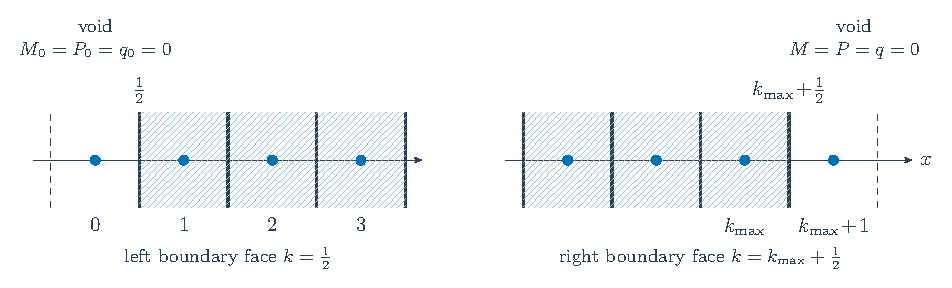
\includegraphics[width=0.72\textwidth]{hc_void_v1.pdf}
  \caption{Void boundaries (cartoon). One empty ghost cell on each end of the mesh; the real material is hatched.\label{fig:void}}
\end{figure}


\clearpage

\begin{tcolorbox}[breakable]
\textbf{One Cycle, In Order:}\vspace{.5em}
\begin{itemize}
\item[a.] Velocity \bm{$u^{n+\frac{1}{2}}$} on every face, from \bm{$P^n$}, \bm{$q^n$}
\item[b.] Positions \bm{$x^{n+1}$}, then densities \bm{$\rho^{n+1}$}
\item[c.] Energies \bm{$e^{n+1}$}, from \bm{$P^n$}, \bm{$q^n$}, \bm{$u^{n\pm\frac{1}{2}}$}
\item[d.] Pressures \bm{$P^{n+1}$} (keep them \bm{$\ge 0$}; \texttt{bitwhiz}: the spall rule), then sound speeds \bm{$c^{n+1}$}
\item[e.] Viscosities \bm{$q^{n+1}$}, then the next time step \bm{$\Delta t^{n+1}$}
\item[f.] Write output if needed; \bm{$n\leftarrow n+1$}; repeat until the termination time\vspace{.5em}
\item Check, \hspace{3mm} total mass \bm{$\sum_k M_k$} is exact; total energy \bm{$\sum_k M_k\left(e_k+\frac{1}{2}\bar{u}_k^2\right)$} and momentum \bm{$\sum_k M_k\bar{u}_k$} should hold to round-off and truncation error (\texttt{bitwhiz} reports both every cycle)
\end{itemize}
\end{tcolorbox}

\;\\

\begin{tcolorbox}[breakable]
\textbf{bitwhiz: Where This Lives in the Code:}\vspace{.5em}
\begin{itemize}
\item Steps, \hspace{3mm} Step 0 \bm{$\rightarrow$} \texttt{maincode} sections 5--6; \hspace{2mm} Step 1 \bm{$\rightarrow$} \texttt{face\_step} (loop 1) and the density in \texttt{cell\_step} (loop 2); \hspace{2mm} Step 2 energy \bm{$\rightarrow$} \texttt{cell\_step}; \hspace{2mm} EOS, spall rule, \bm{$c$}, \bm{$q$}, \bm{$\Delta t_k$} \bm{$\rightarrow$} \texttt{cell\_state}, \texttt{cell\_dt} (loop 3); \hspace{2mm} EOS formulas \bm{$\rightarrow$} \texttt{eos\_mod}; \hspace{2mm} the cycle and \bm{$\Delta t_{CFL}$} \bm{$\rightarrow$} \texttt{maincode} section 7\vspace{.5em}
\item Database Slots, \hspace{3mm} one array \texttt{database(nvar,imax)}; faces and cells alternate along the second index\vspace{.5em}\\
\begin{center}\small
\begin{tabular}{llllll}
\toprule
\multicolumn{2}{l}{On the faces} & \multicolumn{2}{l}{In the cells} & \multicolumn{2}{l}{Material (cells)} \\
\midrule
\bm{$x^{n+1}$} & \texttt{jx} & \bm{$M_k$} & \texttt{jm} & \bm{$\rho_0$} & \texttt{jr0} \\
\bm{$x^{n}$} & \texttt{jx\_old} & \bm{$\rho^{n+1}$}, \bm{$\rho^n$} & \texttt{jrho}, \texttt{jrho\_old} & \bm{$c_0$} & \texttt{jc0} \\
\bm{$u^{n+\frac{1}{2}}$} & \texttt{ju} & \bm{$e^{n+1}$}, \bm{$e^n$} & \texttt{je}, \texttt{je\_old} & \bm{$s_1$}, \bm{$s_2$} & \texttt{js1}, \texttt{js2} \\
\bm{$u^{n-\frac{1}{2}}$} & \texttt{ju\_old} & \bm{$P$}, \bm{$q$}, \bm{$c$} & \texttt{jp}, \texttt{jq}, \texttt{jc} & \bm{$\Gamma_0$} & \texttt{jg0} \\
node mass & \texttt{jmf} & \bm{$\mathcal{D}$} & \texttt{jdam} & \bm{$P_{sp}$} & \texttt{jsp} \\
\bottomrule
\end{tabular}
\end{center}\vspace{.5em}
\item Index Rule, \hspace{3mm} cell \bm{$k$} is at \bm{$i=2k+1$}, face \bm{$k+\frac{1}{2}$} at \bm{$i=2k+2$}; ghost cells are \bm{$k=0$} and \bm{$k_{\max}+1$} \hspace{7mm} (\texttt{shock\_mod}: \texttt{icell}, \texttt{iface})\vspace{.5em}
\item Units, \hspace{3mm} exactly the set above; \texttt{bitwhiz} has no conversion factors
\end{itemize}
\end{tcolorbox}

\end{document}
